\documentclass{article}
\usepackage[spanish]{babel}
\usepackage[numbers,sort&compress]{natbib}
\usepackage[T1]{fontenc}
\usepackage[ansinew]{inputenc}
\usepackage{graphicx}
\usepackage{url}
\usepackage{caption}
\usepackage{float}
\usepackage{subcaption}
\usepackage{caption}
\usepackage{listings}
\usepackage{amsmath}
\usepackage{natbib}



\title {Frentes de Pareto}
\author{Oscar Qui\~nonez}

\begin{document}

\maketitle
 
\section{Objetivo}\label{met}

En el presente trabajo se muestran los frentes de Pareto tambi\'en conocido como eficiencia de Pareto, el cual nos ayuda para la optimizaci\'on de problemas con m\'ultiples criterios, en el que puede haber contradicci\'on entre ellos, por ejemplo, al mejorar uno de ellos, los dem\'as empeoran y tambi\'en en sentido contrario, para este trabajo se siguieron las instrucciones \cite{satuelisa} dadas en clase. 

\section{Metodolog\'ia}\label{met}

Usando como herramienta Python 3.7 se tom\'o el c\'odigo proporcionado en clase \cite{doctora} en el que se pide graficar las funciones objetivo con valores entre 2 y 12 adem\'as de usar una cantidad $n$ de soluciones, que para este caso son 150. Al proceder con la simulaci\'on se pudieron ver cambios en las 12 gr\'aficas de tipo viol\'in que fueron generadas.

\section{Resultados y Discusi\'on}\label{res}

En las gr\'aficas mostradas en la figura 1 se representan cada una de las funciones objetivo, estas nos indican que conforme su aumento, tambi\'en aumentan las soluciones no dominadas, sin embargo, ninguna llega claramente al 100\%. Todas las gr\'aficas se pueden ver en el repositorio de Github \cite{yo}. 

\begin{figure}[H]
       \centering
       \begin{subfigure}[b]{0.30\linewidth}
           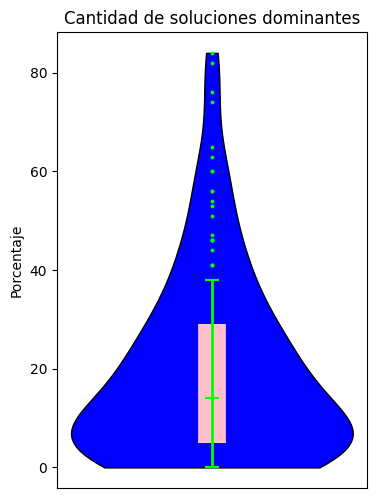
\includegraphics[width=\linewidth]{tareaonce_violin1.png}
           \caption{Funci\'on objetivo 2}
           \label{fig:westminster_lateral}
        \end{subfigure}
        \begin{subfigure}[b]{0.30\linewidth}
           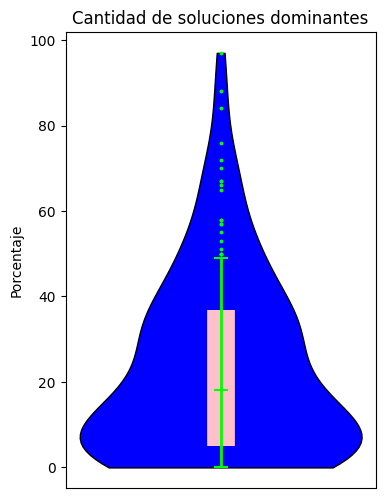
\includegraphics[width=\linewidth]{tareaonce_violin2.png}
           \caption{Funci\'on objetivo 3}
           \label{fig:westminster_lateral}
        \end{subfigure}
        \begin{subfigure}[b]{0.30\linewidth}
           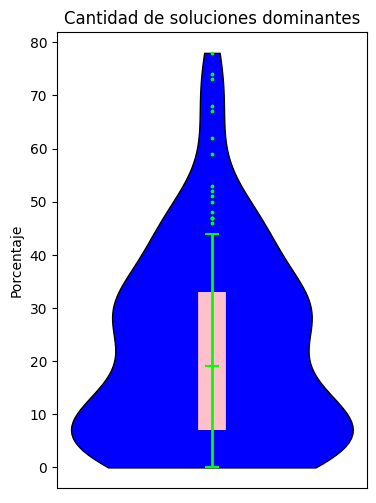
\includegraphics[width=\linewidth]{tareaonce_violin3.png}
           \caption{Funci\'on objetivo 4}
           \label{fig:westminster_lateral}
        \end{subfigure}
        \begin{subfigure}[b]{0.30\linewidth}
           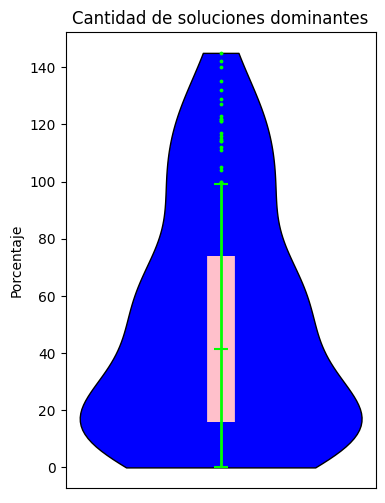
\includegraphics[width=\linewidth]{tareaonce_violin4.png}
           \caption{Funci\'on objetivo 5}
           \label{fig:westminster_lateral}
        \end{subfigure}
         \begin{subfigure}[b]{0.30\linewidth}
           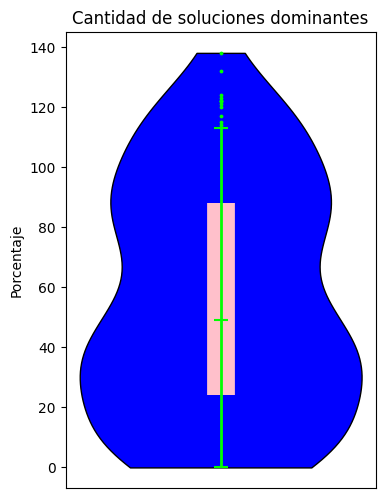
\includegraphics[width=\linewidth]{tareaonce_violin5.png}
           \caption{Funci\'on objetivo 6}
           \label{fig:westminster_lateral}
        \end{subfigure}  
        \begin{subfigure}[b]{0.30\linewidth}
           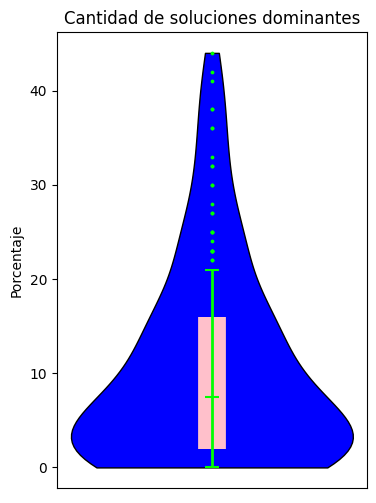
\includegraphics[width=\linewidth]{tareaonce_violin6.png}
           \caption{Funci\'on objetivo 7}
           \label{fig:westminster_lateral}
        \end{subfigure}
        \begin{subfigure}[b]{0.30\linewidth}
           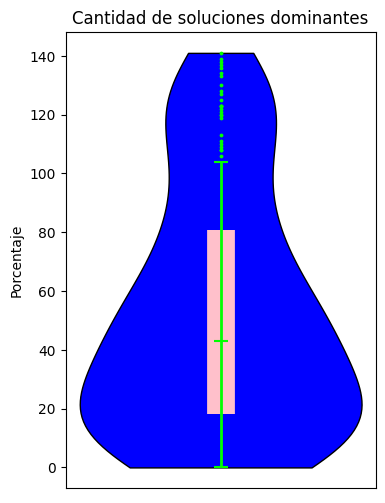
\includegraphics[width=\linewidth]{tareaonce_violin7.png}
           \caption{Funci\'on objetivo 8}
           \label{fig:westminster_lateral}
        \end{subfigure}
        \begin{subfigure}[b]{0.30\linewidth}
           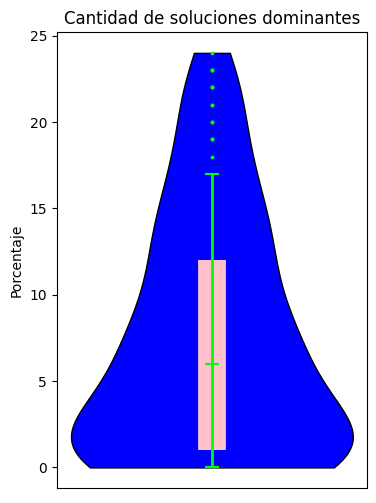
\includegraphics[width=\linewidth]{tareaonce_violin8.png}
           \caption{Funci\'on objetivo 9}
           \label{fig:westminster_lateral}
        \end{subfigure}
        \begin{subfigure}[b]{0.30\linewidth}
           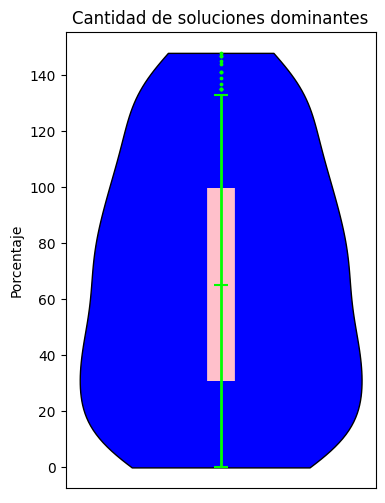
\includegraphics[width=\linewidth]{tareaonce_violin9.png}
           \caption{Funci\'on objetivo 10}
           \label{fig:westminster_lateral}
        \end{subfigure}
        \begin{subfigure}[b]{0.30\linewidth}
           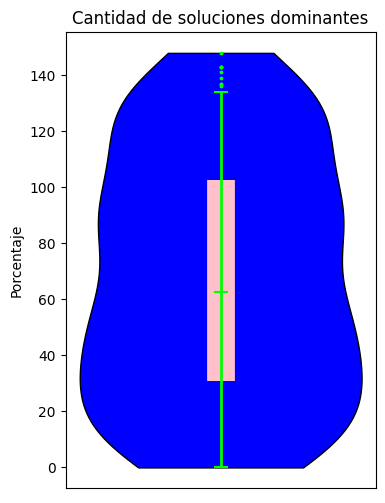
\includegraphics[width=\linewidth]{tareaonce_violin10.png}
           \caption{Funci\'on objetivo 11}
           \label{fig:westminster_lateral}
        \end{subfigure}
        \begin{subfigure}[b]{0.30\linewidth}
           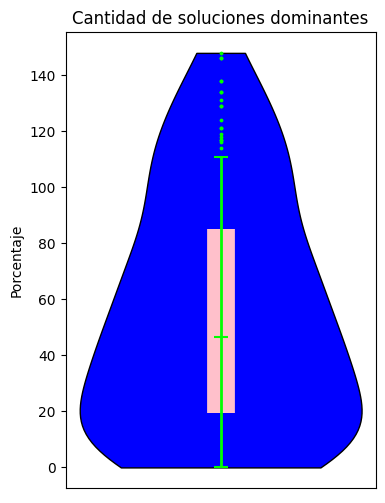
\includegraphics[width=\linewidth]{tareaonce_violin11.png}
           \caption{Funci\'on objetivo 12}
           \label{fig:westminster_lateral}
        \end{subfigure}
        \caption{Simulaci\'on usando 150 soluciones}
        \label{fig:westminster}
\end{figure}

\newpage
\section{Conclusi\'on}

Se puede inferir que el efecto de las 12 muestras objetivos es debido a que se usaron 150 soluciones y tal vez con una cantidad mucho mayor se podr\'ia ver una tendencia hacia el 100\%, esto no se realiz\'o debido a la capacidad del equipo utilizado, pero cabe aclarar que este mismo efecto s\'i nos servir\'ia en una simulaci\'on multicriterio como lo son los frentes de Pareto. 

\bibliography{tareaonce}
\bibliographystyle{unsrtnat}

\end{document}
